\protect\hyperlink{main-nav}{≡} \protect\hyperlink{close-nav}{×}

\hypertarget{section-1.7-exponential-functions}{%
\section{Section 1.7: Exponential
Functions}\label{section-1.7-exponential-functions}}

Consider these two companies:

\begin{itemize}
\tightlist
\item
  Company A has 100 stores, and expands by opening 50 new stores a year
\item
  Company B has 100 stores, and expands by increasing the number of
  stores by 50\% of their total each year.
\end{itemize}

Company A is exhibiting linear growth. In linear growth, we have a
constant rate of change -- a constant number that the output increased
for each increase in input. For company A, the number of new stores per
year is the same each year.

Company B is different -- we have a percent rate of change rather than a
constant number of stores/year as our rate of change. To see the
significance of this difference compare a 50\% increase when there are
100 stores to a 50\% increase when there are 1000 stores:

\begin{itemize}
\tightlist
\item
  100 stores, a 50\% increase is 50 stores in that year.
\item
  1000 stores, a 50\% increase is 500 stores in that year.
\end{itemize}

Calculating the number of stores after several years, we can clearly see
the difference in results.

\begin{longtable}[]{@{}lll@{}}
\toprule
\endhead
Years & Company A & Company B\tabularnewline
2 & 200 & 225\tabularnewline
4 & 300 & 506\tabularnewline
6 & 400 & 1139\tabularnewline
8 & 500 & 2563\tabularnewline
10 & 600 & 5767\tabularnewline
\bottomrule
\end{longtable}

\begin{figure}
\centering
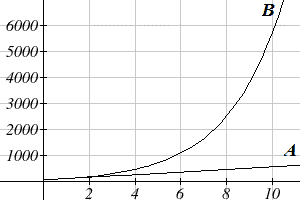
\includegraphics{images/image072.png}
\caption{Graphs of data from A and B, with B fit to a curve.}
\end{figure}

This percent growth can be modeled with an exponential function.

\hypertarget{exponential-function}{%
\paragraph{Exponential Function}\label{exponential-function}}

An \textbf{exponential growth or decay function} is a function that
grows or shrinks at a constant percent growth rate. The equation can be
written in the form \textbackslash{}{[}
f(x)=a(1+r)\^{}x\textbackslash{}{]} or \textbackslash{}{[}
f(x)=ab\^{}x\textbackslash{}{]} where \textbackslash{}( b=1+r
\textbackslash{}).

Where

\begin{itemize}
\tightlist
\item
  \textbackslash{}(a\textbackslash{}) is the initial or starting value
  of the function,
\item
  \textbackslash{}(r\textbackslash{}) is the percent growth or decay
  rate, written as a decimal,
\item
  \textbackslash{}(b\textbackslash{}) is the growth factor or growth
  multiplier. Since powers of negative numbers behave strangely, we
  limit \textbackslash{}(b\textbackslash{}) to positive values.
\end{itemize}

To view this video please enable JavaScript, and consider upgrading to a
web browser that \href{http://videojs.com/html5-video-support/}{supports
HTML5 video}

\hypertarget{example-1}{%
\paragraph{Example 1}\label{example-1}}

India's population was 1.14 billion in the year 2008 and is growing by
about 1.34\% each year. Write an exponential function for India's
population, and use it to predict the population in 2020.

Using 2008 as our starting time (\textbackslash{}(t =
0\textbackslash{})), our initial population will be 1.14 billion. Since
the percent growth rate was 1.34\%, our value for
\textbackslash{}(r\textbackslash{}) is 0.0134.

Using the basic formula for exponential growth
\textbackslash{}(f(x)=a(1+r)\^{}x\textbackslash{}) we can write the
formula,
\textbackslash{}{[}f(t)=1.14(1+0.0134)\^{}\{t\}\textbackslash{}{]}

To estimate the population in 2020, we evaluate the function at
\textbackslash{}(t = 12\textbackslash{}), since 2020 is 12 years after
2008:
\textbackslash{}{[}f(t)=1.14(1+0.0134)\^{}\{12\}\textbackslash{}approx
1.337 \textbackslash{}text\{ billion people in
2020.\}\textbackslash{}{]}

\hypertarget{example-2}{%
\paragraph{Example 2}\label{example-2}}

A certificate of deposit (CD) is a type of savings account offered by
banks, typically offering a higher interest rate in return for a fixed
length of time you will leave your money invested. If a bank offers a 24
month CD with an annual interest rate of 1.2\% compounded monthly, how
much will a \$1000 investment grow to over those 24 months?

First, we must notice that the interest rate is an annual rate, but is
compounded monthly, meaning interest is calculated and added to the
account monthly. To find the monthly interest rate, we divide the annual
rate of 1.2\% by 12 since there are 12 months in a year: 1.2\%/12 =
0.1\%. Each month we will earn 0.1\% interest. From this, we can set up
an exponential function, with our initial amount of \$1000 and a growth
rate of \textbackslash{}( r = 0.001\textbackslash{}), and our input
\textbackslash{}(m\textbackslash{}) measured in months:
\textbackslash{}{[}f(m)=1000\textbackslash{}left(1+\textbackslash{}frac\{0.012\}\{12\}\textbackslash{}right)\^{}m=1000(1.001)\^{}\{m\}\textbackslash{}{]}

After 24 months, the account will have grown to \textbackslash{}(
f(24)=1000(1.001)\^{}\{24\}\textbackslash{}approx
\textbackslash{}\$1024.28 \textbackslash{}).

\hypertarget{example-3}{%
\paragraph{Example 3}\label{example-3}}

Bismuth-210 is an isotope that radioactively decays by about 13\% each
day, meaning 13\% of the remaining Bismuth-210 transforms into another
atom (polonium-210 in this case) each day. If you begin with 100 mg of
Bismuth-210, how much remains after one week?

With radioactive decay, instead of the quantity increasing at a percent
rate, the quantity is decreasing at a percent rate. Our initial quantity
is \textbackslash{}(a = 100\textbackslash{}) mg, and our growth rate
will be negative 13\%, since we are decreasing: \textbackslash{}( r =
-0.13\textbackslash{}). This gives the equation \textbackslash{}{[}
Q(d)=100(1-0.13)\^{}d=100(0.87)\^{}d.\textbackslash{}{]} This can also
be explained by recognizing that if 13\% decays, then 87 \% remains.

After one week, 7 days, the quantity remaining would be
\textbackslash{}( Q(7)=100(0.87)\^{}7=37.73 \textbackslash{}) mg of
Bismuth-210 remains.

\hypertarget{example-4}{%
\paragraph{Example 4}\label{example-4}}

\textbackslash{}(T(q)\textbackslash{}) represents the total number of
Android smart phone contracts, in thousands, held by a certain Verizon
store region measured quarterly since January 1, 2010. Interpret all of
the parts of the equation \textbackslash{}( T(2)=86(1.64)\^{}2=231.3056
\textbackslash{}) .

Interpreting this from the basic exponential form, we know that 86 is
our initial value. This means that on Jan. 1, 2010 this region had
86,000 Android smart phone contracts. Since \textbackslash{}(b = 1 + r =
1.64\textbackslash{}), we know that every quarter the number of smart
phone contracts grows by 64\%. \textbackslash{}(T(2) =
231.3056\textbackslash{}) means that in the second quarter (or at the
end of the second quarter) there were approximately 231,305 Android
smart phone contracts.

When working with exponentials, there is a special constant we must talk
about. It arises when we talk about things growing continuously, such as
continuous compounding, or natural phenomena like radioactive decay that
happen continuously.

\hypertarget{eulers-number-e}{%
\paragraph{Euler's Number:
\textbackslash{}(e\textbackslash{})}\label{eulers-number-e}}

\textbackslash{}{[}e\textbackslash{}approx 2.718282\textbackslash{}{]}

Because \textbackslash{}(e\textbackslash{}) is often used as the base of
an exponential, most scientific and graphing calculators have a button
that can calculate powers of \textbackslash{}(e\textbackslash{}),
usually labeled . Some computer software instead defines a function
exp(x), where exp(x) = \textbackslash{}(e\^{}x\textbackslash{}). Since
calculus studies continuous change, we will almost always use the
\textbackslash{}(e\textbackslash{})-based form of exponential equations
in this course.

\hypertarget{continuous-growth-formula}{%
\paragraph{Continuous Growth Formula}\label{continuous-growth-formula}}

\textbf{Continuous growth} can be calculated using the formula
\textbackslash{}{[}f(x)=ae\^{}\{rx\}\textbackslash{}{]} where

\begin{itemize}
\tightlist
\item
  \textbackslash{}(a\textbackslash{}) is the starting amount,
\item
  \textbackslash{}(r\textbackslash{}) is the continuous growth rate.
\end{itemize}

\hypertarget{example-5}{%
\paragraph{Example 5}\label{example-5}}

Radon-222 decays at a continuous rate of 17.3\% per day. How much will
100mg of Radon-222 decay to in 3 days?

Since we are given a continuous decay rate, we use the continuous growth
formula. Since the substance is decaying, we know the growth rate will
be negative: \textbackslash{}(r = -0.173\textbackslash{}),
\textbackslash{}( f(3)=100e\^{}\{-0.173(3)\}\textbackslash{}approx
59.512 \textbackslash{}) mg of Radon-222 will remain.

\hypertarget{graphs-of-exponential-functions}{%
\subsection{Graphs of Exponential
Functions}\label{graphs-of-exponential-functions}}

\hypertarget{graphical-features-of-exponential-functions}{%
\paragraph{Graphical Features of Exponential
Functions}\label{graphical-features-of-exponential-functions}}

Graphically, in the function \textbackslash{}( f(x)=ab\^{}x
\textbackslash{}).

\begin{itemize}
\tightlist
\item
  \textbackslash{}(a\textbackslash{}) is the vertical intercept of the
  graph.
\item
  \textbackslash{}(b\textbackslash{}) determines the rate at which the
  graph grows:

  \begin{itemize}
  \tightlist
  \item
    the function will increase if \textbackslash{}(b \textbackslash{}gt
    1\textbackslash{}),
  \item
    the function will decrease if \textbackslash{}(0 \textbackslash{}lt
    b \textbackslash{}lt 1\textbackslash{}).
  \end{itemize}
\item
  The graph will have a horizontal asymptote at \textbackslash{}(y =
  0\textbackslash{}).
\item
  The graph will be concave up if \textbackslash{}(a \textbackslash{}gt
  0\textbackslash{}); concave down if \textbackslash{}(a
  \textbackslash{}lt 0\textbackslash{}).
\item
  The domain of the function is all real numbers.
\item
  The range of the function is \textbackslash{}(
  (0,\textbackslash{}infty) \textbackslash{}) if \textbackslash{}(a
  \textbackslash{}gt 0\textbackslash{}), and \textbackslash{}(
  (-\textbackslash{}infty, 0) \textbackslash{}) if \textbackslash{}(a
  \textbackslash{}lt 0\textbackslash{}).
\end{itemize}

When sketching the graph of an exponential function, it can be helpful
to remember that the graph will pass through the points
\textbackslash{}((0, a)\textbackslash{}) and \textbackslash{}((1,
ab)\textbackslash{}).

The value \textbackslash{}(b\textbackslash{}) will determine the
function's long run behavior:

\begin{itemize}
\tightlist
\item
  If \textbackslash{}(b \textbackslash{}gt 1\textbackslash{}), as
  \textbackslash{}( x\textbackslash{}to\textbackslash{}infty
  \textbackslash{}), \textbackslash{}(
  f(x)\textbackslash{}to\textbackslash{}infty \textbackslash{}), and as
  \textbackslash{}( x\textbackslash{}to -\textbackslash{}infty
  \textbackslash{}), \textbackslash{}( f(x)\textbackslash{}to 0
  \textbackslash{}).
\item
  If \textbackslash{}(0 \textbackslash{}lt b \textbackslash{}lt
  1\textbackslash{}), as \textbackslash{}(
  x\textbackslash{}to\textbackslash{}infty \textbackslash{}),
  \textbackslash{}( f(x)\textbackslash{}to 0 \textbackslash{}), and as
  \textbackslash{}( x\textbackslash{}to -\textbackslash{}infty
  \textbackslash{}), \textbackslash{}( f(x)\textbackslash{}to
  \textbackslash{}infty \textbackslash{}).
\end{itemize}

\hypertarget{example-6}{%
\paragraph{Example 6}\label{example-6}}

Sketch a graph of \textbackslash{}(
f(x)=4\textbackslash{}left(\textbackslash{}frac\{1\}\{3\}\textbackslash{}right)\^{}x
\textbackslash{})

This graph will have a vertical intercept at (0,4), and pass through the
point \textbackslash{}(
\textbackslash{}left(1,\textbackslash{}frac\{4\}\{3\}
\textbackslash{}right) \textbackslash{}). Since \textbackslash{}(b
\textbackslash{}lt 1\textbackslash{}), the graph will be decreasing
towards zero. Since \textbackslash{}(a \textbackslash{}gt
0\textbackslash{}), the graph will be concave up.

\begin{figure}
\centering
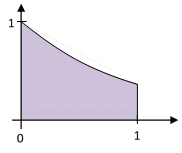
\includegraphics{images/image073.png}
\caption{}
\end{figure}

We can also see from the graph the long run behavior: as
\textbackslash{}( x\textbackslash{}to\textbackslash{}infty
\textbackslash{}), \textbackslash{}( f(x)\textbackslash{}to 0
\textbackslash{}), and as \textbackslash{}( x\textbackslash{}to
-\textbackslash{}infty \textbackslash{}), \textbackslash{}(
f(x)\textbackslash{}to \textbackslash{}infty \textbackslash{}).

To get a better feeling for the effect of
\textbackslash{}(a\textbackslash{}) and
\textbackslash{}(b\textbackslash{}) on the graph, examine the sets of
graphs below. The first set shows various graphs, where
\textbackslash{}(a\textbackslash{}) remains the same and we only change
the value for \textbackslash{}(b\textbackslash{}). Notice that the
closer the value of \textbackslash{}(b\textbackslash{}) is to 1, the
less steep the graph will be.

\begin{figure}
\centering
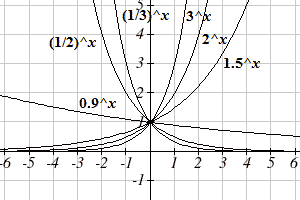
\includegraphics{images/image074.png}
\caption{Changing the value of \textbackslash{}( b \textbackslash{}).}
\end{figure}

In the next set of graphs, \textbackslash{}(a\textbackslash{}) is
altered and our value for \textbackslash{}(b\textbackslash{}) remains
the same.

\begin{figure}
\centering
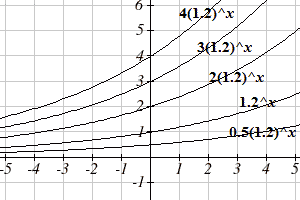
\includegraphics{images/image075.png}
\caption{Changing the value of \textbackslash{}( a \textbackslash{}).}
\end{figure}

Notice that changing the value for a changes the vertical intercept.
Since \textbackslash{}(a\textbackslash{}) is multiplying the
\textbackslash{}(b\^{}x\textbackslash{}) term,
\textbackslash{}(a\textbackslash{}) acts as a vertical stretch factor,
not as a shift. Notice also that the long run behavior for all of these
functions is the same because the growth factor did not change and none
of these \textbackslash{}(a\textbackslash{}) values introduced a
vertical flip.

Try it for yourself using this applet:

\hypertarget{applet_container}{}

\hypertarget{example-7}{%
\paragraph{Example 7}\label{example-7}}

Match each equation with its graph.

\begin{itemize}
\tightlist
\item
  \textbackslash{}( f(x)=2(1.3)\^{}x \textbackslash{})
\item
  \textbackslash{}( g(x)=2(1.8)\^{}x \textbackslash{})
\item
  \textbackslash{}( h(x)=4(1.3)\^{}x \textbackslash{})
\item
  \textbackslash{}( k(x)=4(0.7)\^{}x \textbackslash{})
\end{itemize}

\begin{figure}
\centering
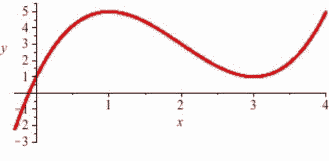
\includegraphics{images/image076.png}
\caption{}
\end{figure}

The graph of \textbackslash{}(k(x)\textbackslash{}) is the easiest to
identify, since it is the only equation with a growth factor less than
one, which will produce a decreasing graph. The graph of
\textbackslash{}(h(x)\textbackslash{}) can be identified as the only
growing exponential function with a vertical intercept at (0,4). The
graphs of \textbackslash{}(f(x)\textbackslash{}) and
\textbackslash{}(g(x)\textbackslash{}) both have a vertical intercept at
(0,2), but since \textbackslash{}(g(x)\textbackslash{}) has a larger
growth factor, we can identify it as the graph increasing faster.

\begin{figure}
\centering
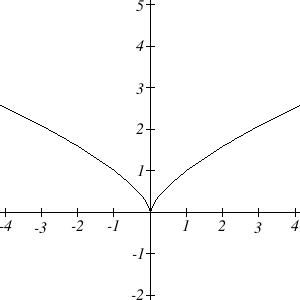
\includegraphics{images/image077.png}
\caption{}
\end{figure}

\begin{longtable}[]{@{}ll@{}}
\toprule
\endhead
\href{section.1-6php}{← Previous Section} & \href{section1-8.php}{Next
Section →}\tabularnewline
\bottomrule
\end{longtable}
